%2025 - 4a
%
\section{04a : Espace vectoriel tangent (suite)}

%{Vitesse d'une courbe en un point}%(rappel)
\subsection{rappels}
Une variété topologique de dimension n un ensemble de point munie d'une topologie et d'un atlas : (M, $\mc{O}$, $\mc{A}$).
Un atlas est un ensemble de cartes, une carte est une application homéomorphe d'un ouvert autour d'un point dans  $\mb{R}^n$ :
\[
\mc{A} = \{ (\mc{U}, x) : \mc{U} \to \mb{R}^n\}
\]
\[
\mathscr{A} = \{ (\mathscr{U}, x) : \mathscr{O} \to \mb{R}^n\}
\]
Si l'atlas est restreint aux cartes qui peuvent être reliées par des transformations infiniment dérivables, on a une variété différentielle : (M, $\mc{O}$, $\mc{A}_\infty$).

 = localement (autour de chaque point), la variété est isomorphe à $\mb{R}^n$ : $\mc{A}$ est un ensemble de cartes, les cartes étant des applications homéomorphe d'un ouvert autour de chaque point dans $\mb{R}^n$ qui permet de donner des coordonnées aux points

\begin{minipage}[c]{.5\linewidth}
\[
\begin{array}{ l c l l }
 \gamma : & \mb{R} & \to & M \\ 
  & \lambda & \mapsto & \gamma(\lambda) \\
\end{array}
\]
\end{minipage}
\hfill
\begin{minipage}[c]{.5\linewidth}
\[
\begin{array}{ l c l l }
 \mr{V}_{\gamma,p} : & \mc{C}^\infty(M) & \to & \mb{R} \\ 
  & f & \mapsto & {v}_{\gamma,p}(f)=(f\circ\gamma)'|_{\lambda_0} \\
\end{array}
\]
\end{minipage}


\[
\gamma(\lambda_0)=p\in M
\]


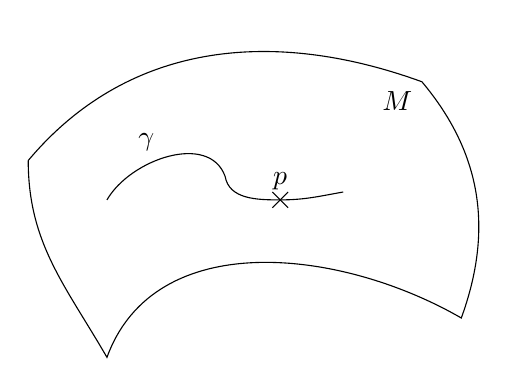
\begin{tikzpicture}
\draw(-3, 1) to[out=50, in=160] (2,2) node[below left]{$M$}
to[out=-50, in=70] (2.5,-1)
to[out=150, in=70] (-2,-1.5)
to[out=120, in=-90] (-3, 1); % Espace
%
\draw(-1.5,1) node[above]{$\gamma 	$};
\draw(-2,0.5) to[out=60, in=110] (-0.5,0.8)
to[out=-80, in=180]  (0.2,0.5) node[above]{$p$}
to[out=0, in=190] (1,0.6); % Courbe
%
\draw(0.1,0.6) -- (0.3,0.4);
\draw(0.1,0.4) -- (0.3,0.6);
\end{tikzpicture}

\[
(f_1+f_2)(x)=f_1(x)+f_2(x)
 \qquad 
(\lambda f)(x)=\lambda f(x)
\]

\section{Espace vectoriel tangent}
Par définition, l'espace vectoriel tangent à M au point p est :
\[
T_pM = \{ {v}_{\gamma,p}\ |\ \gamma : I \to M  \}
\]
x, y étant deux cartes de M, on a :
\[
\gamma : I \to M \qquad x : M \to \mb{R}^n \qquad y : M \to \mb{R}^n
\]
et
\[
x \circ \gamma : I \to \mb{R}^n \qquad y \circ \gamma : I \to \mb{R}^n
\]
et
\[
y \circ x^{-1} : \mb{R}^n \to \mb{R}^n
\]

\begin{minipage}[c]{.45\linewidth}
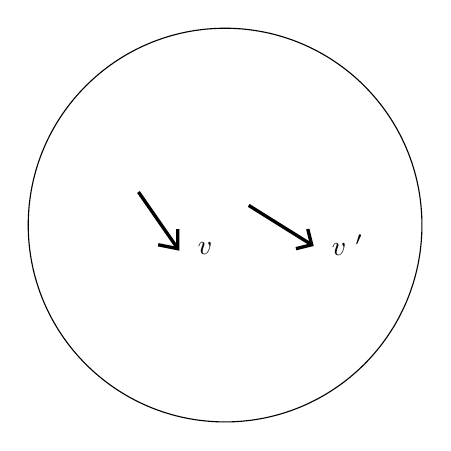
\begin{tikzpicture} % "THE GLOBE" showcase
\def\R{2.5} \def\angEl{35} % sphere radius, elevation angle
\draw (0,0) circle (\R);%\filldraw[ball] (0,0) circle (\R);
\foreach \t in {-80,-50,...,80} { \DrawLatitudeCircle[\R]{\t} }
\foreach \t in {10,-35,...,-150} { \DrawLongitudeCircle[\R]{\t} }
\draw[very thick](-1.1,0.42) -- (-0.6,-0.3)node[right]{$\ \mv{v}$};
\draw[very thick](-0.85,-0.25) -- (-0.6,-0.3) -- (-0.6,-0.05);
\draw[very thick](0.3,0.25) -- (1.1,-0.25)node[right]{$\ \mv{v}\ '$};
\draw[very thick](0.9,-0.3) -- (1.1,-0.25) -- (1.05,-0.05);
\end{tikzpicture}
\end{minipage}
\hfill
\begin{minipage}[c]{.45\linewidth}
\end{minipage}

\begin{minipage}[c]{.45\linewidth}
$(T_pM, +, \cdot)$ est un espace vectoriel.

$+$ : addition de vitesse

$\cdot$ : multiplication par un scalaire

\end{minipage}
 \begin{proof}
\hfill
\begin{minipage}[c]{.45\linewidth}
Soit $\gamma_1$ et $\gamma_2$ deux courbes lisses ($\in \mc{C}^\infty$). On étudie $\mr{V}_{\gamma_1,p}+\mr{V}_{\gamma_2,p}$ :
\[
f \mapsto(\mr{V}_{\gamma_1,p}+\mr{V}_{\gamma_2,p})(f) =
\mr{V}_{\gamma_1,p}(f)+\mr{V}_{\gamma_2,p}(f)
\]
\end{minipage}

\begin{minipage}[c]{.45\linewidth}
\[
\lambda \in \mb{R}, \ \mr{V}_\gamma \in T_{p\,}M
\]
\[
\lambda \cdot \mr{V}_\gamma
\]
\end{minipage}
\hfill
\begin{minipage}[c]{.45\linewidth}
\[
\begin{array}{ l c l l }
 \mr{V}_{\gamma,p} : & \mc{C}^\infty(M) & \to & \mb{R} \\ 
  & f & \mapsto & {v}_{\gamma,p}(f)=(f\circ\gamma)'|_{\lambda_0} \\
\end{array}
\]
\end{minipage}

\end{proof}
%{"Reparamétrage" d'une courbe}%
%{Espace vectoriel tangent, TpM : addition de deux vitesses et multiplication par un scalaire}%
%{Courbes coordonnées (d'une carte donnée) et vitesses associées}%
%{Base de TpM associée à une carte donnée}%
%{Notation importante : "dérivée partielle d'une fonction", représentée dans une carte}%
